\documentclass[10pt,a4paper]{article}

\usepackage[utf8]{inputenc}
\usepackage[T1]{fontenc}
\usepackage[brazil]{babel}
\usepackage[margin=2.0cm,headheight=22pt]{geometry}
\usepackage{helvet}
\renewcommand{\familydefault}{\sfdefault}
\usepackage{mathastext} % Padroniza todas as fontes matemáticas e numéricas
\usepackage{microtype}
\usepackage{xcolor}
\usepackage{graphicx}
\usepackage{booktabs}
\usepackage{array}
\usepackage{float}
\usepackage[most]{tcolorbox}
\usepackage{fancyhdr}
\usepackage{lastpage}
\usepackage{titlesec}
\usepackage{setspace}
\usepackage{hyperref}

% Paleta de Cores Civic-Tech / The Broadsheet (design-rules.md)
\definecolor{PetroleoDark}{HTML}{06333D}
\definecolor{PetroleoMedium}{HTML}{005B68}
\definecolor{Terracota}{HTML}{C84B31}
\definecolor{SlateText}{HTML}{1F2937}
\definecolor{SlateMuted}{HTML}{6B7280}
\definecolor{BorderGray}{HTML}{D8CCC0}
\definecolor{BgSoft}{HTML}{FAF8F5}
\definecolor{TagEsquerda}{HTML}{C84B31}
\definecolor{TagDireita}{HTML}{005B68}

\setstretch{1.10}
\setlength{\parskip}{0.28em}
\setlength{\parindent}{0pt}

% Configuração de títulos
\titleformat{\section}
  {\Large\bfseries\color{PetroleoDark}}
  {\thesection.}{0.6em}{}
  [\vspace{-0.3em}{\color{PetroleoMedium}\rule{\textwidth}{1.2pt}}\vspace{0.15em}]

\titleformat{\subsection}
  {\large\bfseries\color{PetroleoMedium}}
  {\thesubsection}{0.5em}{}

\titleformat{\subsubsection}
  {\normalsize\bfseries\color{PetroleoDark}}
  {\thesubsubsection}{0.5em}{}

% Configuração de hiperlinks
\hypersetup{
    colorlinks=true,
    linkcolor=PetroleoMedium,
    urlcolor=PetroleoMedium,
    citecolor=PetroleoDark
}

% Cabeçalho e Rodapé
\pagestyle{fancy}
\fancyhf{}
\fancyhead[L]{\small\color{SlateMuted}\textbf{Relatório Metodológico} \textbar\ Posicionamento Partidário e Quiz}
\fancyhead[R]{\small\color{SlateMuted}Página \thepage\ de \pageref{LastPage}}
\renewcommand{\headrulewidth}{0.5pt}
\renewcommand{\footrulewidth}{0pt}
\renewcommand{\headrule}{\hbox to\headwidth{\color{BorderGray}\leaders\hrule height \headrulewidth\hfill}}

% Estilo de Caixas Informativas (tcolorbox)
\tcbset{
    editorialbox/.style={
        enhanced,
        colback=BgSoft,
        colframe=PetroleoMedium,
        arc=2.0mm,
        left=5mm,
        right=5mm,
        top=3.5mm,
        bottom=3.5mm,
        boxrule=1.0pt,
        leftrule=4.0pt,
        shadow={0.6mm}{-0.6mm}{0mm}{black!5}
    }
}

\begin{document}

% ======================================================================
% PÁGINA 1: CABEÇALHO INSTITUCIONAL E RESUMO EXECUTIVO APLICADO
% ======================================================================
\begin{flushleft}
    {\huge\textbf{\color{PetroleoDark} Relatório Metodológico}}\\[0.2em]
    {\LARGE\textbf{\color{PetroleoMedium} Posicionamento Partidário e Fundamentação do Quiz Eleitoral (VAA)}}\\[0.5em]
    {\color{BorderGray}\rule{\textwidth}{1.6pt}}\\[0.3em]
    
    \begin{tabular*}{\textwidth}{@{\extracolsep{\fill}}l l l l@{}}
        \textbf{\color{PetroleoDark} Autor:} Vinícius Pinon & \textbf{\color{PetroleoDark} Data:} Setembro de 2026 & \textbf{\color{PetroleoDark} Versão:} 2.6 & \textbf{\color{PetroleoDark} Plataforma:} \href{https://emquemeuvoto.onrender.com}{emquemeuvoto.onrender.com} \\
    \end{tabular*}
\end{flushleft}

\vspace{0.6em}

\begin{tcolorbox}[editorialbox, title={\bfseries\large Resumo Executivo}]
Este documento detalha os critérios metodológicos adotados para estimar o posicionamento político-partidário e fundamentar empiricamente o questionário de afinidade eleitoral (quiz). A metodologia estabelece uma abordagem descritiva, reproduzível e auditável, ancorada exclusivamente em dados observáveis e pesquisas consagradas da Ciência Política:

\begin{itemize}\setlength{\itemsep}{0.25em}
    \item \textbf{Triangulação de Três Fontes Independentes:} Para mitigar distorções e evitar a dependência de narrativas conjunturais ou fontes isoladas, a plataforma combina três pilares consolidados da Ciência Política brasileira:
    \begin{enumerate}\setlength{\itemsep}{0.15em}
        \item \textit{A Visão dos Próprios Parlamentares:} \textbf{Brazilian Legislative Survey (BLS / Oxford e FGV)}, pesquisa direta com deputados e senadores em exercício;
        \item \textit{A Avaliação de Especialistas:} \textbf{Levantamento da ABCP (Bolognesi, Ribeiro e Codato, DADOS)}, consulta sistemática a pesquisadores e cientistas políticos;
        \item \textit{O Comportamento Concreto:} \textbf{GPS Partidário (DeltaFolha, 2026)}, mensuração empírica multidimensional estruturada em cinco eixos (votações nominais no plenário, migrações na janela partidária, frentes parlamentares, coligações eleitorais e doações financeiras).
    \end{enumerate}
    \item \textbf{Régua Contínua Padronizada (0 a 100):} As escalas foram linearmente convertidas para uma métrica uniforme de 0,0 (Extrema-Esquerda) a 100,0 (Extrema-Direita), organizada em 7 faixas conceituais orientativas para facilitar a interpretação pelo cidadão.
    \item \textbf{Transparência Metodológica para Partidos Estreantes:} Legendas recém-registradas no TSE ou sem histórico de votações consolidadas com bancada legislativa são documentadas com sinalização formal explícita sobre a extensão de dados disponível, sem estimativas arbitrárias.
    \item \textbf{Perguntas Baseadas em Dados Reais do Congresso:} As 7 afirmações do quiz eleitoral foram formuladas a partir de microdados reais de 109 parlamentares federais na Pesquisa Legislativa Brasileira (BLS 9), assegurando correspondência com as clivagens substantivas do debate legislativo nacional.
    \item \textbf{Autonomia do Cidadão e Finalidade Informativa:} A plataforma não possui caráter prescritivo nem busca definir o voto do usuário. Seu papel é exclusivamente orientativo, permitindo ao cidadão compreender os posicionamentos médios das legendas e filtrar candidatos livremente.
\end{itemize}
\end{tcolorbox}

\vspace{0.8em}
\begin{center}
    {\color{BorderGray}\rule{0.4\textwidth}{0.8pt}}\\[0.6em]
    \small\color{SlateMuted}Documento técnico de transparência metodológica e comunicação com a sociedade civil.
\end{center}

\clearpage

% ======================================================================
% PÁGINA 2: SEÇÃO 1, SEÇÃO 2 E DIMENSÕES ANALÍTICAS
% ======================================================================
\section{Por que Triangular o Posicionamento dos Partidos?}

No sistema político brasileiro, classificar legendas partidárias a partir de um único critério analítico introduz vieses sistemáticos:
\begin{itemize}\setlength{\itemsep}{0.12em}
    \item \textbf{Estatutos Partidários:} Em geral contêm declarações de princípios abrangentes e genéricas, pouco elucidativas sobre a disciplina de bancada no plenário.
    \item \textbf{Discursos de Lideranças:} Respondem frequentemente a conveniências conjunturais e estratégias discursivas imediatas de períodos eleitorais.
    \item \textbf{Apoio a Governos no Presidencialismo de Coalizão:} A adesão de partidos a governos federais envolve partilha de cargos, ministérios e emendas parlamentares, fenômeno que nem sempre expressa afinidade ideológica substantiva.
\end{itemize}

A triangulação de três fontes independentes atenua ruídos idiossincráticos e captura facetas complementares da vida partidária:

\vspace{0.4em}
\begin{center}
\small
\setlength{\tabcolsep}{4pt}
\renewcommand{\arraystretch}{1.22}
\begin{tabular*}{\textwidth}{@{\extracolsep{\fill}}p{3.8cm} p{4.6cm} p{7.6cm}@{}}
\toprule
\textbf{Dimensão Analítica} & \textbf{Fonte Metodológica} & \textbf{Objeto Observado na Prática} \\
\midrule
\textbf{Olhar dos Representantes} & BLS (Power \& Zucco, Oxford/FGV) & Como os próprios parlamentares em exercício posicionam a si mesmos e aos seus pares. \\
\textbf{Olhar dos Especialistas} & ABCP (Bolognesi et al., Revista DADOS) & Avaliação sistemática de pesquisadores e professores vinculados à Ciência Política. \\
\textbf{Olhar Comportamental} & DeltaFolha (GPS Partidário, 2026) & Votações nominais na Câmara (IRT), migrações partidárias, frentes e coligações eleitorais. \\
\bottomrule
\end{tabular*}
\end{center}

\vspace{0.8em}

\section{As Três Fontes Metodológicas e o Índice Sintético}

A metodologia integra três estudos independentes consolidados na literatura científica nacional:

\begin{enumerate}\setlength{\itemsep}{0.28em}
    \item \textbf{Pilar 1 — Brazilian Legislative Survey (BLS / Power \& Zucco, Oxford e FGV):} Pesquisa longitudinal de referência internacional que coleta dados diretamente de parlamentares federais desde 1990. Aplica a correção de \textit{Aldrich-McKelvey} para homogeneizar as escalas de percepção dos respondentes contra o problema do funcionamento diferencial dos itens (DIF).
    \item \textbf{Pilar 2 — Levantamento com Especialistas da ABCP (Bolognesi, Ribeiro \& Codato, 2023):} Consulta periódica a centenas de especialistas vinculados à Associação Brasileira de Ciência Política, publicada na revista acadêmica \textit{DADOS}, abrangendo também agremiações de fusão recente e legendas menores.
    \item \textbf{Pilar 3 — GPS Partidário 2026 (DeltaFolha / Folha de S.Paulo, 2026):} Mapeamento empírico multidimensional baseado em cinco dimensões observáveis de dados abertos do Congresso e do TSE: votações nominais no plenário da Câmara dos Deputados (Item Response Theory), migrações de bancada na janela partidária, frentes parlamentares, alianças eleitorais e redes de doadores.
\end{enumerate}

\clearpage

% ======================================================================
% PÁGINA 3: FIGURA 1 E AS 7 FAIXAS CONCEITUAIS
% ======================================================================
\subsection{Arquitetura da Triangulação Metodológica}

\begin{figure}[H]
    \centering
    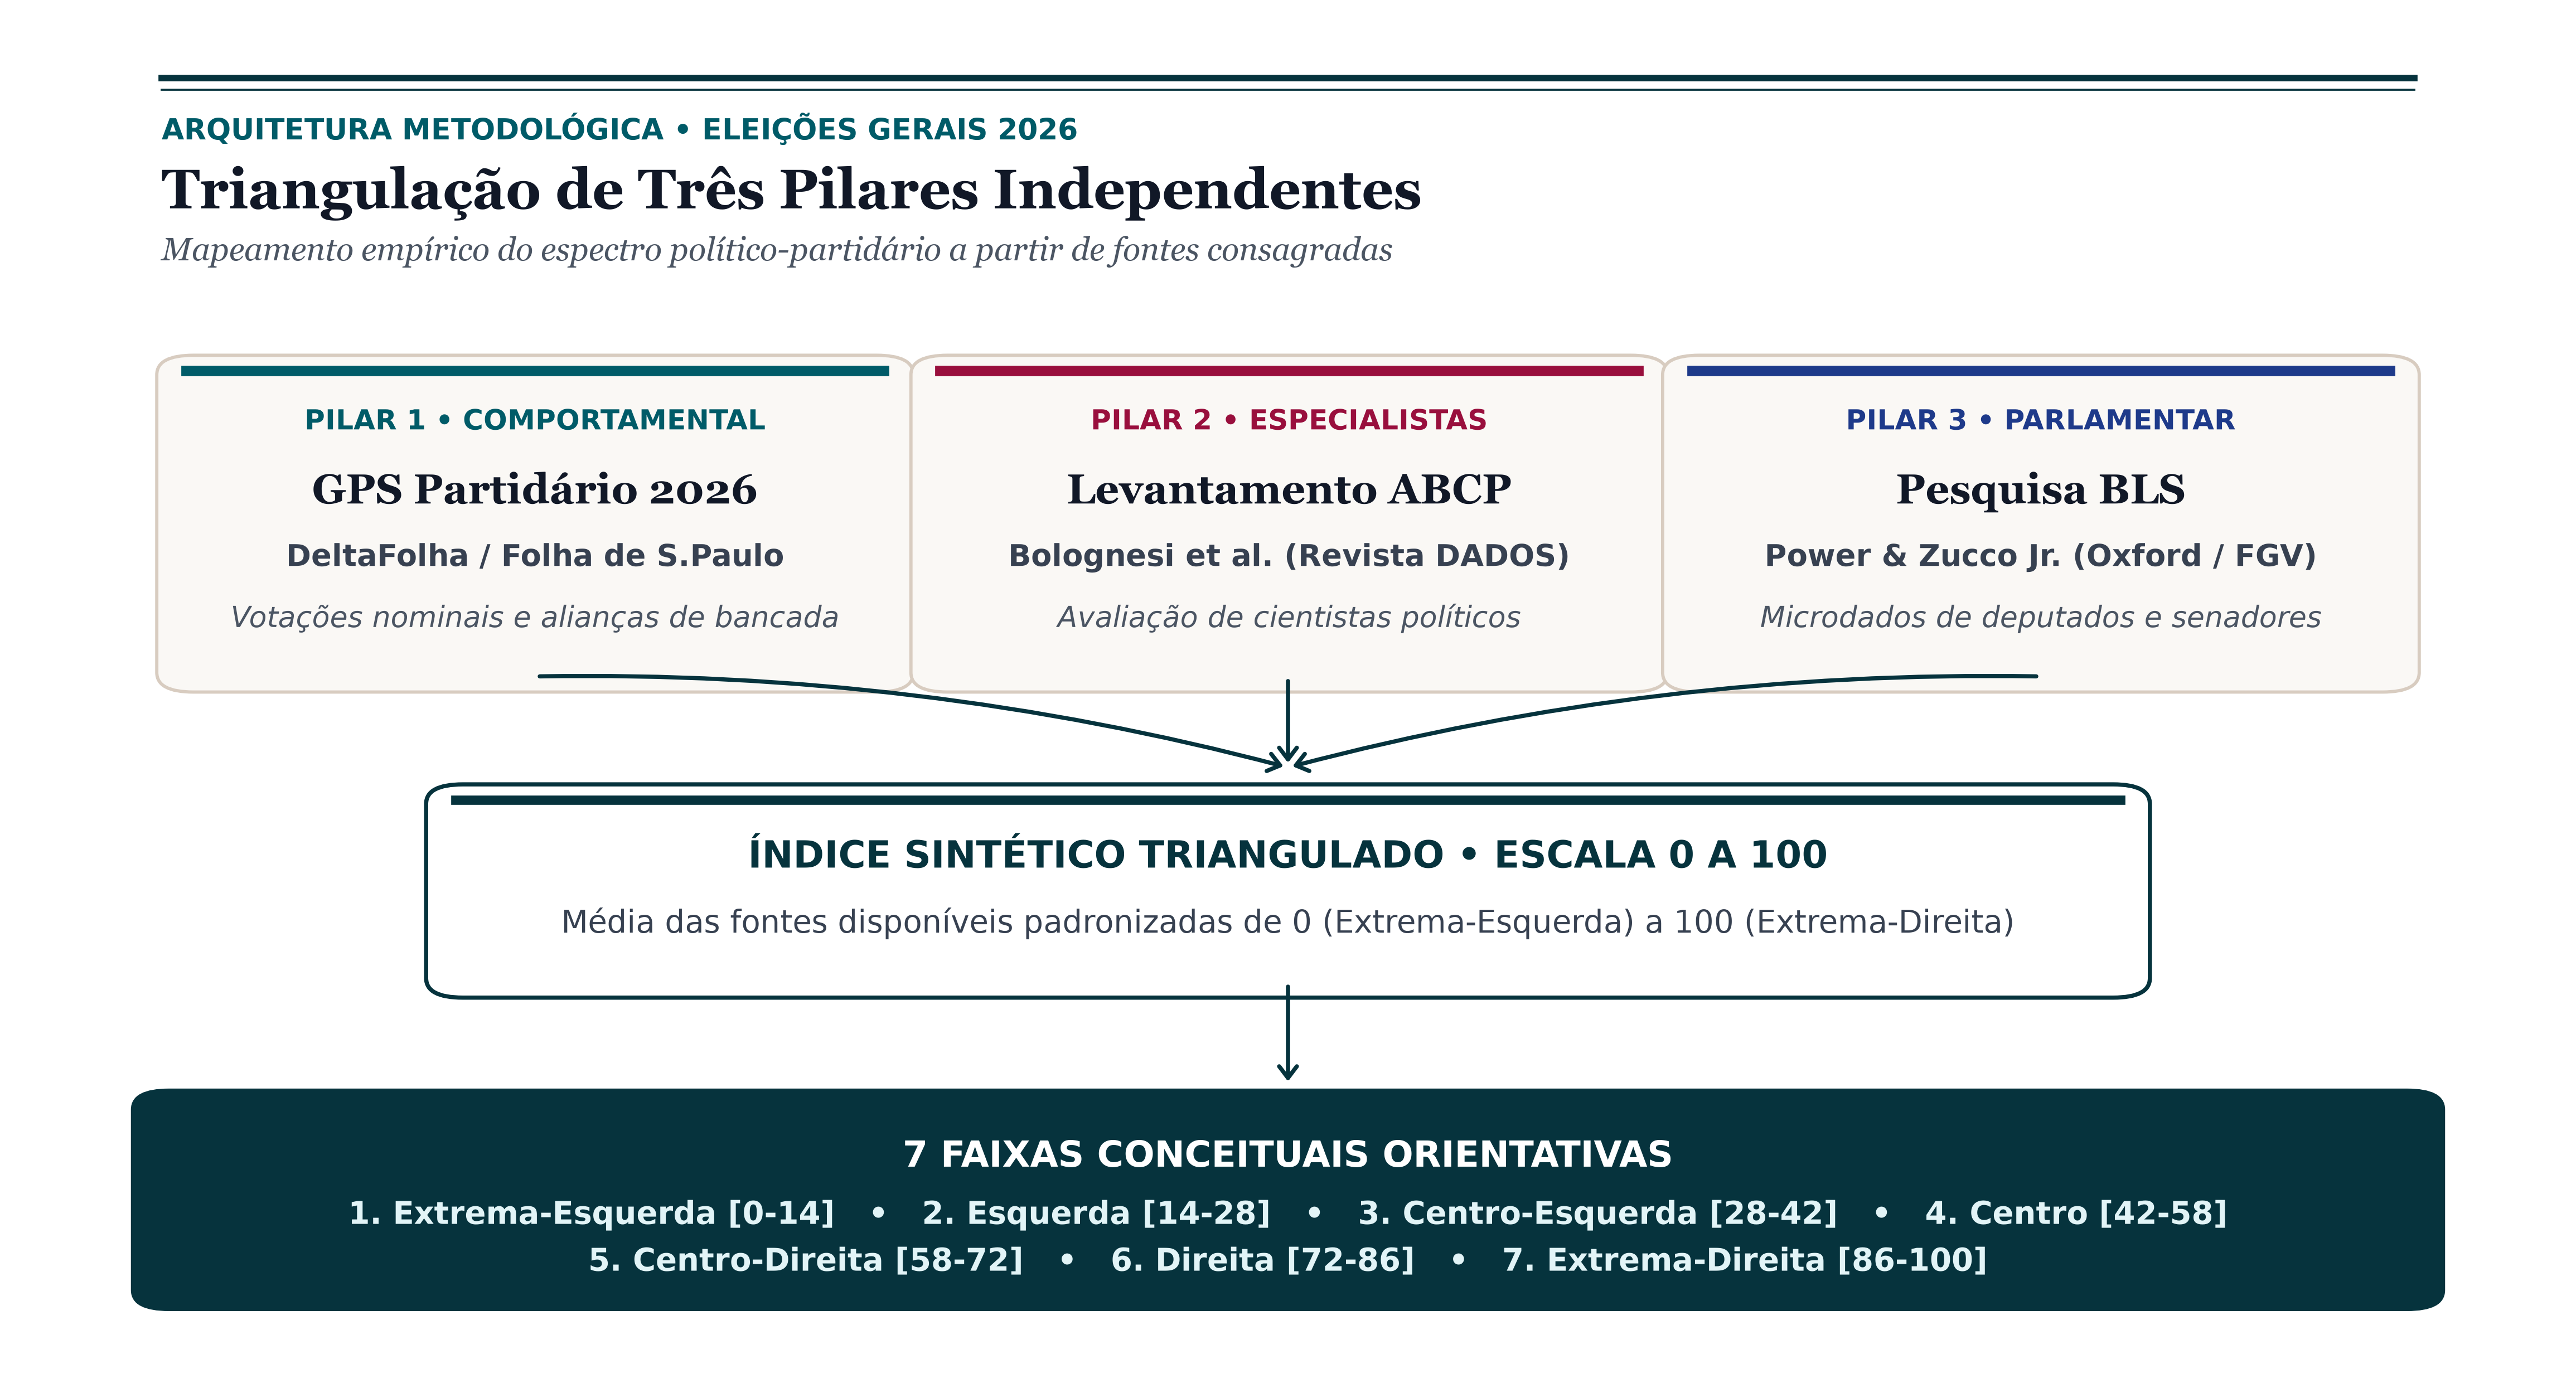
\includegraphics[width=0.96\textwidth]{figures/fluxo_metodologico_triangulacao.png}
    \caption{\textbf{Arquitetura da Triangulação Metodológica:} Integração dos três pilares independentes para o cálculo do Índice Sintético contínuo (0 a 100) e distribuição em 7 faixas conceituais orientativas.}
    \label{fig:fluxo}
\end{figure}

\vspace{0.2em}

\subsection{Cálculo do Índice e as 7 Faixas Orientativas}

Todas as escalas originais foram convertidas para uma métrica uniforme de 0,0 (Extrema-Esquerda) a 100,0 (Extrema-Direita). O \textbf{Índice Sintético Consolidado} é a média aritmética simples das fontes disponíveis para cada partido.

Para orientar a navegação do cidadão na plataforma, o espectro contínuo é organizado em 7 faixas conceituais:

\begin{enumerate}\setlength{\itemsep}{0.22em}
    \item \textbf{Faixa 1 — Extrema-Esquerda (0 a 14):} PSTU (3,1), PCO (5,5), PCB (7,6), UP (10,5).
    \item \textbf{Faixa 2 — Esquerda (14 a 28):} PSOL (10,3), PCdoB (13,1), PT (17,8).
    \item \textbf{Faixa 3 — Centro-Esquerda (28 a 42):} REDE (24,1), PSB (30,3), PDT (34,4), PV (36,3).
    \item \textbf{Faixa 4 — Centro (42 a 58):} Avante (54,3), MDB (55,1), Solidariedade (55,9), PSD (59,3), Cidadania (59,4), Mobiliza (61,7).
    \item \textbf{Faixa 5 — Centro-Direita (58 a 72):} Agir (64,4), PSDB (66,8), Podemos (70,8), PP (74,2).
    \item \textbf{Faixa 6 — Direita (72 a 86):} PRD (74,1), PMB/Democrata (75,0), Republicanos (76,5), União Brasil (77,2), DC (82,3).
    \item \textbf{Faixa 7 — Extrema-Direita (86 a 100):} PRTB (84,2), PL (86,1), NOVO (90,0), Missão (92,1).
\end{enumerate}

\clearpage

% ======================================================================
% PÁGINA 4: FIGURA 2 (ESPECTRO POLÍTICO-PARTIDÁRIO 2026)
% ======================================================================
\subsection{O Espectro Político-Partidário Brasileiro (2026)}

A Figura~\ref{fig:espectro} apresenta a distribuição espacial das 29 legendas partidárias registradas perante a Justiça Eleitoral, comparando as estimativas empíricas de cada pilar com o Índice Sintético Consolidado.

\vspace{0.3em}

\begin{figure}[H]
    \centering
    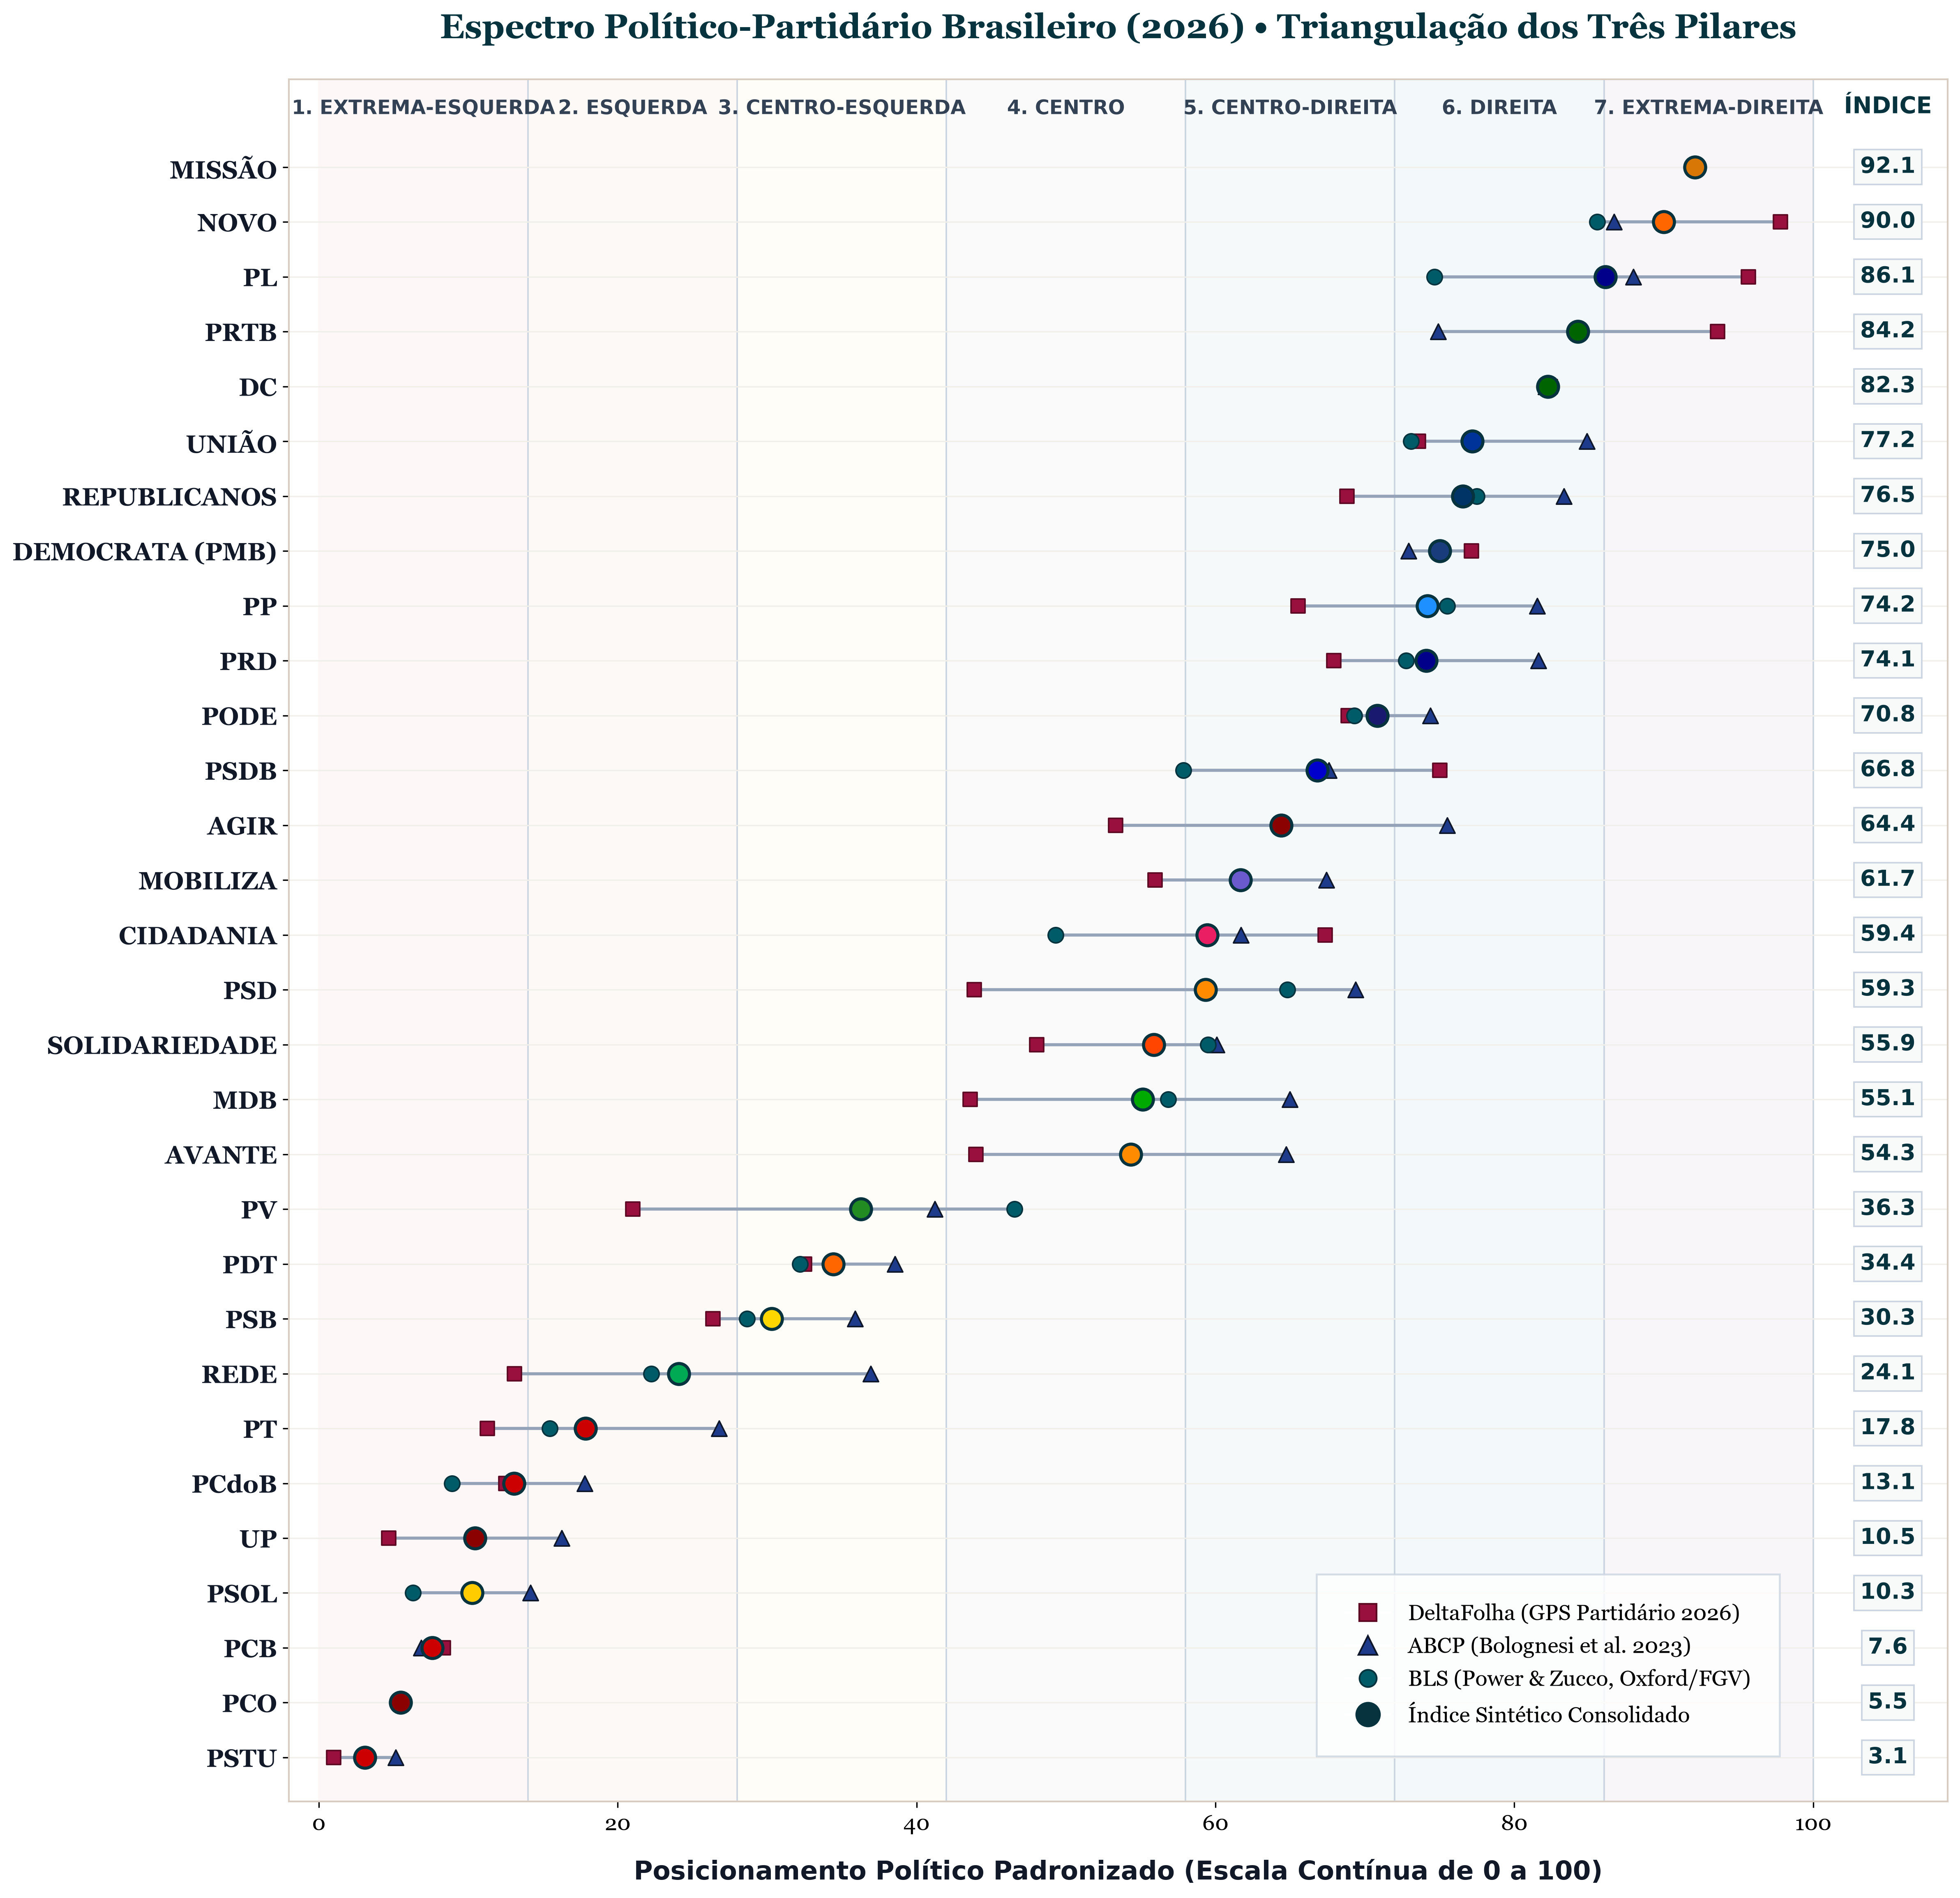
\includegraphics[width=0.92\textwidth]{figures/espectro_partidario_2026.png}
    \caption{\textbf{Espectro Político-Partidário Brasileiro (2026):} Comparação entre as notas do DeltaFolha (2026), Levantamento ABCP (2022) e BLS (Waves 1--9) com o Índice Sintético Consolidado em escala contínua (0 a 100).}
    \label{fig:espectro}
\end{figure}

\clearpage

% ======================================================================
% PÁGINA 5: TABELA 1 CONSOLIDADA (PADRÃO ABNT ESTREITO / PÁGINA COMPLETA)
% ======================================================================
\subsection{Tabela Consolidada das Legendas Partidárias (Norma ABNT)}

A Tabela~\ref{tab:partidos} consolida as pontuações individuais de cada estudo e o índice sintético final das legendas processadas pela plataforma, diagramada segundo os padrões formais de apresentação tabular da ABNT/IBGE (ausência de linhas verticais, cabeçalho e rodapé limpos):

\begin{table}[H]
\centering
\caption{\textbf{Consolidação do posicionamento dos partidos políticos no espectro nacional (2026)}}
\label{tab:partidos}
\vspace{0.4em}
\setlength{\tabcolsep}{4.0pt}
\scriptsize
\renewcommand{\arraystretch}{1.12}
\begin{tabular*}{\textwidth}{@{\extracolsep{\fill}}l p{5.5cm} r r r r c l@{}}
\toprule
\textbf{Sigla} & \textbf{Nome Oficial perante o TSE} & \textbf{Folha '26} & \textbf{ABCP '22} & \textbf{BLS} & \textbf{Índice} & \textbf{Faixa} & \textbf{Classificação} \\
\midrule
\textbf{PSTU} & Partido Socialista dos Trabalhadores Unificado & 1,0 & 5,1 & --- & \textbf{3,1} & 1 & Extrema-Esquerda \\
\textbf{PCO} & Partido da Causa Operária & --- & 5,5 & --- & \textbf{5,5} & 1 & Extrema-Esquerda \\
\textbf{PCB} & Partido Comunista Brasileiro & 8,3 & 6,9 & --- & \textbf{7,6} & 1 & Extrema-Esquerda \\
\textbf{PSOL} & Partido Socialismo e Liberdade & 10,4 & 14,1 & 6,3 & \textbf{10,3} & 2 & Esquerda \\
\textbf{UP} & Unidade Popular & 4,7 & 16,3 & --- & \textbf{10,5} & 1 & Extrema-Esquerda \\
\textbf{PCdoB} & Partido Comunista do Brasil & 12,5 & 17,8 & 8,9 & \textbf{13,1} & 2 & Esquerda \\
\textbf{PT} & Partido dos Trabalhadores & 11,3 & 26,8 & 15,5 & \textbf{17,8} & 2 & Esquerda \\
\textbf{REDE} & Rede Sustentabilidade & 13,1 & 36,9 & 22,3 & \textbf{24,1} & 3 & Centro-Esquerda \\
\textbf{PSB} & Partido Socialista Brasileiro & 26,4 & 35,9 & 28,6 & \textbf{30,3} & 3 & Centro-Esquerda \\
\textbf{PDT} & Partido Democrático Trabalhista & 32,5 & 38,5 & 32,2 & \textbf{34,4} & 3 & Centro-Esquerda \\
\textbf{PV} & Partido Verde & 21,0 & 41,2 & 46,5 & \textbf{36,3} & 3 & Centro-Esquerda \\
\textbf{AVANTE} & Avante & 44,0 & 64,7 & --- & \textbf{54,3} & 4 & Centro \\
\textbf{MDB} & Movimento Democrático Brasileiro & 43,6 & 65,0 & 56,9 & \textbf{55,1} & 4 & Centro \\
\textbf{SOLIDARIEDADE} & Solidariedade & 48,0 & 60,1 & 59,5 & \textbf{55,9} & 4 & Centro \\
\textbf{PSD} & Partido Social Democrático & 43,9 & 69,4 & 64,8 & \textbf{59,3} & 4 & Centro \\
\textbf{CIDADANIA} & Cidadania & 67,3 & 61,7 & 49,3 & \textbf{59,4} & 4 & Centro \\
\textbf{MOBILIZA} & Mobilização Nacional & 56,0 & 67,4 & --- & \textbf{61,7} & 4 & Centro \\
\textbf{AGIR} & Agir & 53,3 & 75,5 & --- & \textbf{64,4} & 5 & Centro-Direita \\
\textbf{PSDB} & Partido da Social Democracia Brasileira & 75,0 & 67,6 & 57,8 & \textbf{66,8} & 5 & Centro-Direita \\
\textbf{PODE} & Podemos & 68,9 & 74,4 & 69,3 & \textbf{70,8} & 5 & Centro-Direita \\
\textbf{PRD} & Partido Renovação Democrática & 67,9 & 81,6 & 72,8 & \textbf{74,1} & 6 & Direita \\
\textbf{PP} & Progressistas & 65,5 & 81,5 & 75,5 & \textbf{74,2} & 5 & Centro-Direita \\
\textbf{PMB / DEMOCRATA} & Democrata (registro PMB) & 77,1 & 72,9 & --- & \textbf{75,0} & 6 & Direita \\
\textbf{REPUBLICANOS} & Republicanos & 68,8 & 83,3 & 77,5 & \textbf{76,5} & 6 & Direita \\
\textbf{UNIÃO} & União Brasil & 73,6 & 84,8 & 73,1 & \textbf{77,2} & 6 & Direita \\
\textbf{DC} & Democracia Cristã & 82,4 & 82,1 & --- & \textbf{82,3} & 6 & Direita \\
\textbf{PRTB} & Partido Renovador Trabalhista Brasileiro & 93,6 & 74,9 & --- & \textbf{84,2} & 7 & Extrema-Direita \\
\textbf{PL} & Partido Liberal & 95,7 & 88,0 & 74,6 & \textbf{86,1} & 7 & Extrema-Direita \\
\textbf{NOVO} & Partido Novo & 97,8 & 86,7 & 85,6 & \textbf{90,0} & 7 & Extrema-Direita \\
\textbf{MISSÃO} & Partido Missão (em formação) & 92,1 & --- & --- & \textbf{92,1} & 7 & Extrema-Direita$^*$ \\
\bottomrule
\end{tabular*}
\vspace{0.4em}
\raggedright \footnotesize
\textbf{Fonte:} Elaboração própria com base em DeltaFolha (2026), Bolognesi et al. (2023) e Power e Zucco Jr. (2023).\\
\textbf{Nota:} Dados empíricos padronizados na métrica contínua de 0 (Extrema-Esquerda) a 100 (Extrema-Direita). A ausência de valor (---) indica inexistência de medição empírica naquele estudo específico. $^*$O Partido Missão possui mensuração registrada unicamente na dimensão de migração partidária do GPS 2026.
\end{table}

\clearpage

% ======================================================================
% PÁGINA 6: SEÇÃO 3 E FIGURA 3 (RANKING DE CORRELAÇÃO DO BLS 9)
% ======================================================================
\section{Fundamentação Empírica do Quiz Eleitoral (VAA)}

\begin{tcolorbox}[editorialbox, title={\bfseries\small O que é uma VAA?}]
\small \textbf{VAA (\textit{Voting Advice Applications})} é a denominação acadêmica internacional para aplicações digitais de afinidade eleitoral (conhecidas popularmente como ``bússolas eleitorais'' ou ``quizzes políticos''). Sua finalidade é estritamente informativa e pedagógica: confrontar preferências do eleitor com posicionamentos médios conhecidos, auxiliando-o a mapear afinidades e a filtrar opções, sem qualquer juízo normativo ou direcionamento de voto.
\end{tcolorbox}

\vspace{0.3em}

Questionários de afinidade eleitoral frequentemente enfrentam restrições metodológicas por formularem dilemas excessivamente abstratos. Para que as afirmações refletissem clivagens reais da política brasileira, as 7 questões do questionário de afinidade foram selecionadas a partir de microdados reais de 109 parlamentares federais na \textbf{Pesquisa Legislativa Brasileira (BLS 9 / FGV e Oxford)}.

\vspace{0.4em}

\begin{figure}[H]
    \centering
    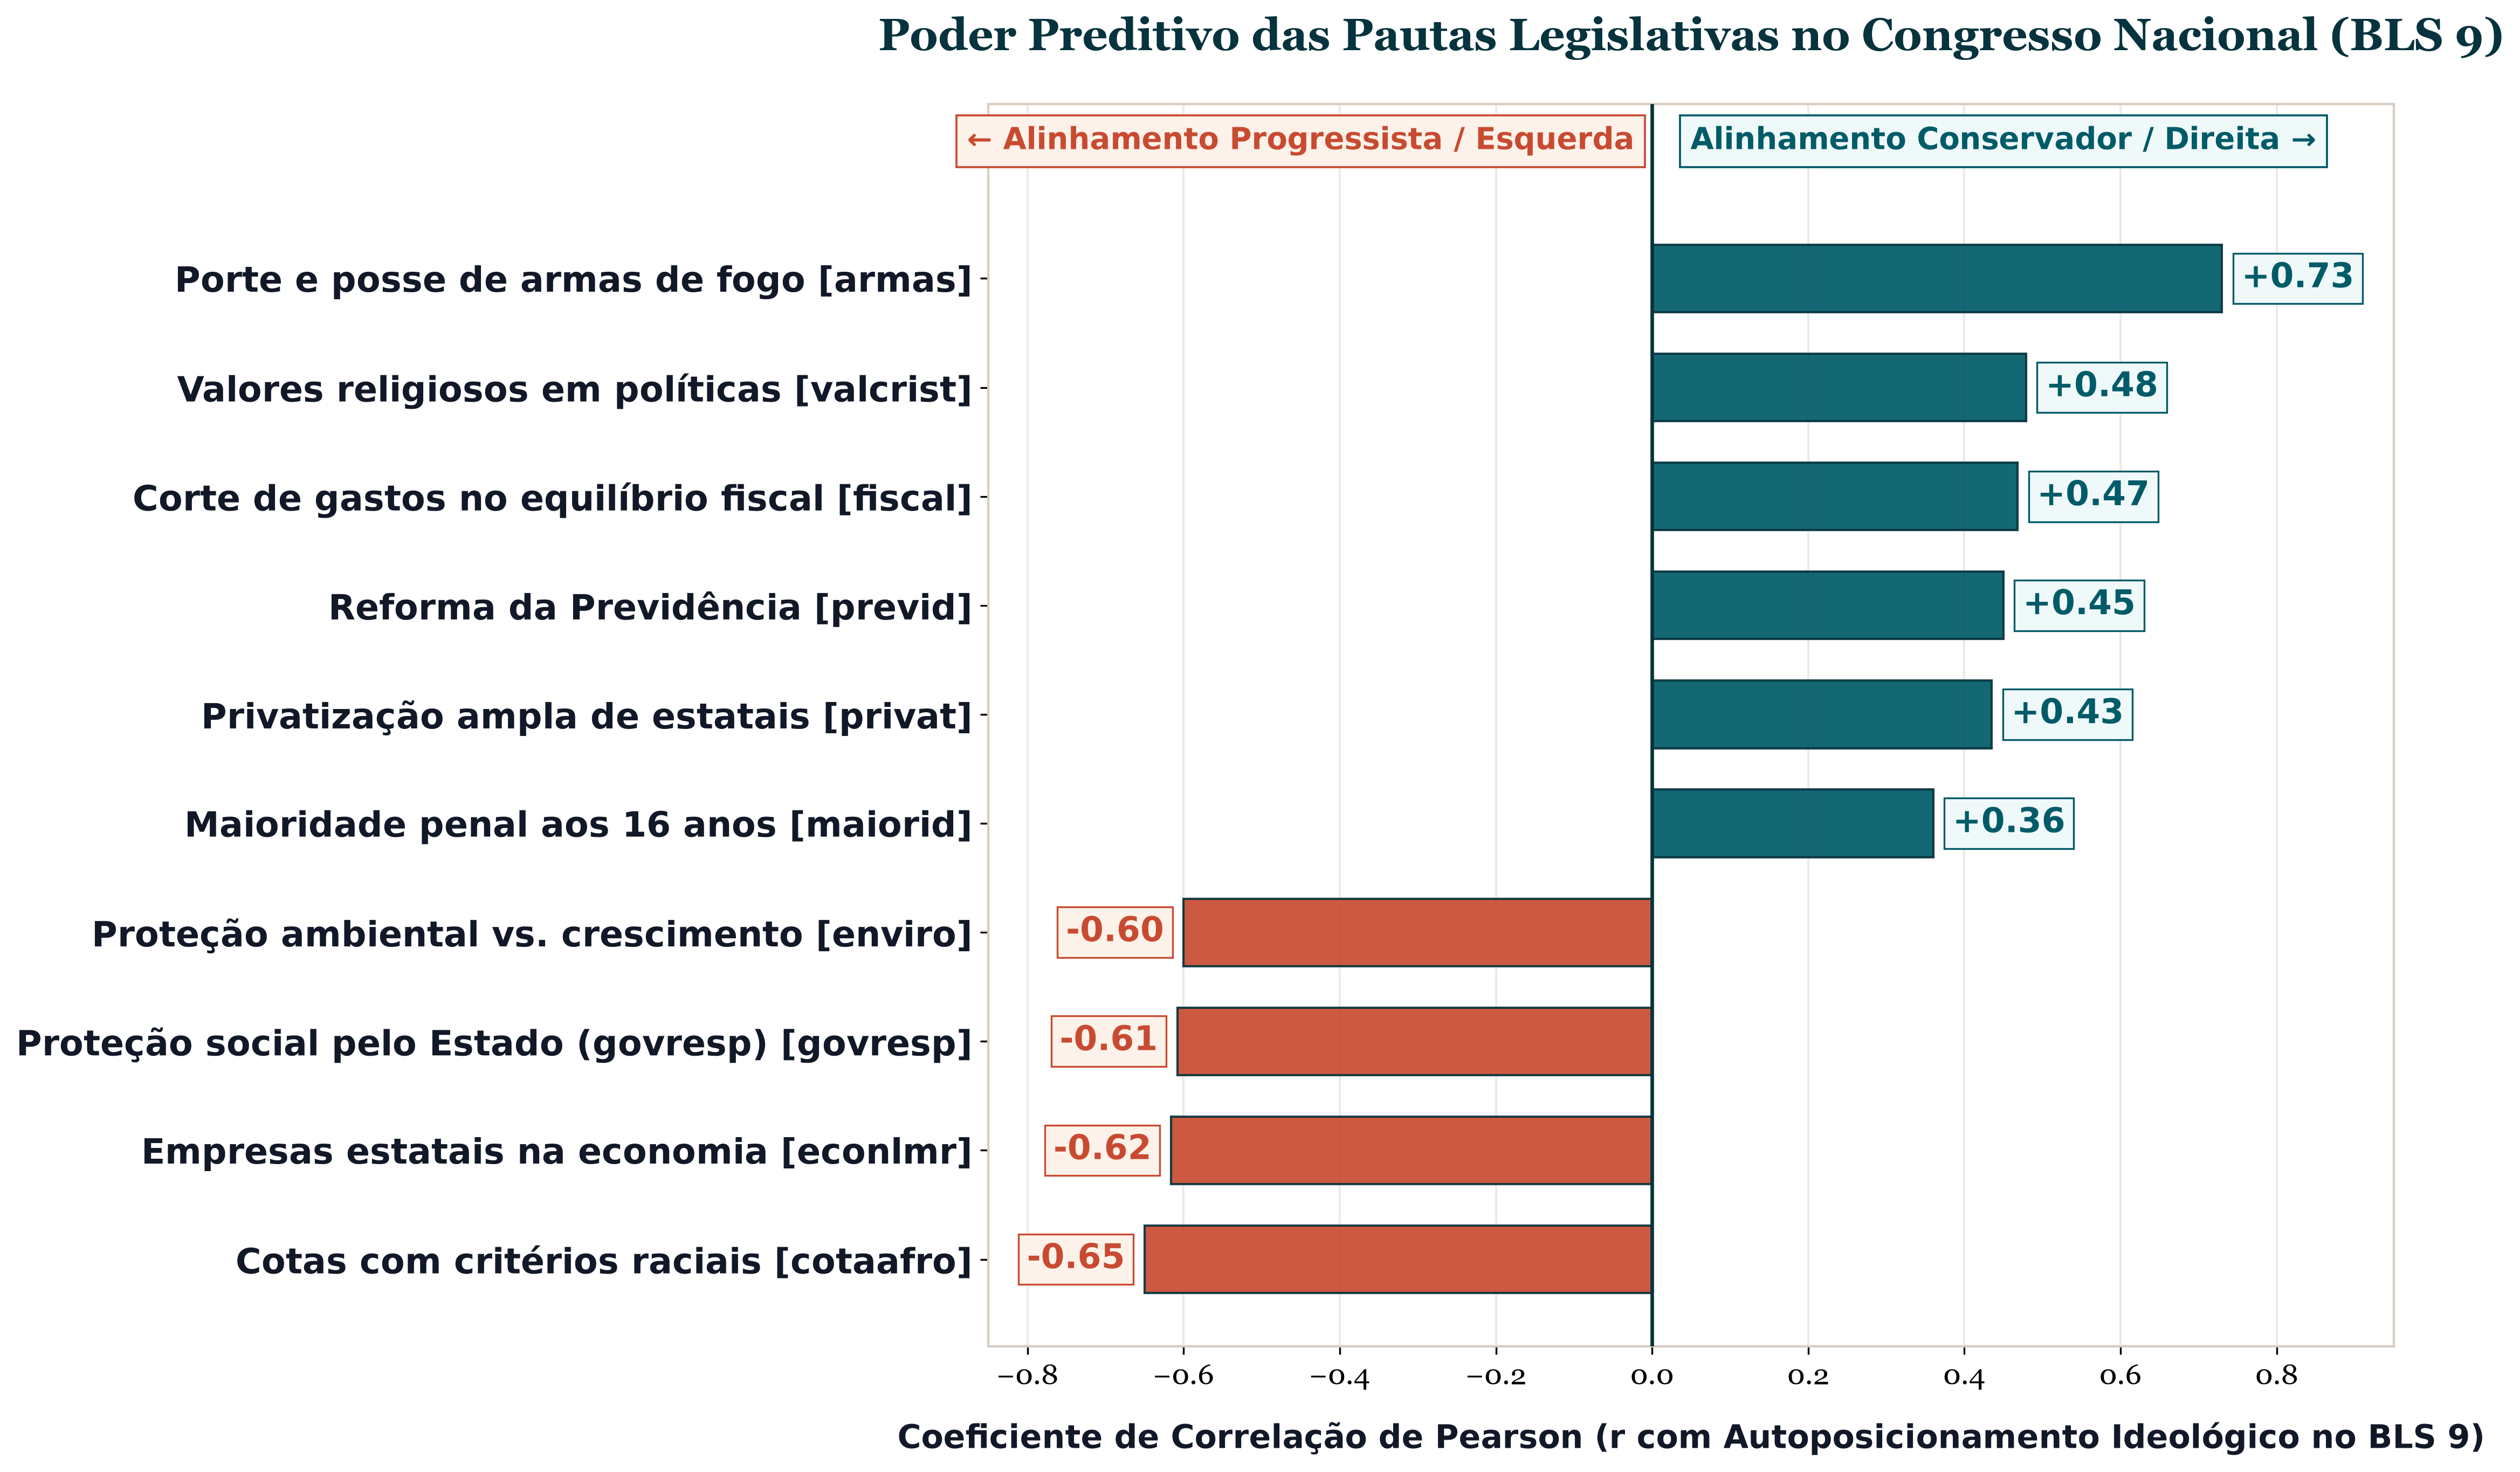
\includegraphics[width=0.96\textwidth]{figures/bls_correlacoes_ranking.png}
    \caption{\textbf{Ranking de Correlação de Pearson (r):} Capacidade de diferenciação empírica dos temas de políticas públicas no Congresso Nacional (BLS 9).}
    \label{fig:correlacoes}
\end{figure}

\clearpage

% ======================================================================
% PÁGINA 7: SEÇÃO 3.1 (CLIVAGENS) E FIGURA 4 (DISPERSÃO BLS 9)
% ======================================================================
\subsection{As Grandes Clivagens no Parlamento Brasileiro}

A análise empírica dos microdados do BLS aponta que há eixos temáticos correlacionados com o posicionamento ideológico dos parlamentares e das legendas partidárias no Brasil:
\begin{enumerate}\setlength{\itemsep}{0.10em}
    \item \textbf{Acesso a Armas de Fogo (\texttt{armas}, $r = +0,730$, $N = 109$):} O tema com maior poder discriminatório no Congresso. A flexibilização do armamento civil correlaciona-se expressivamente com o campo de direita.
    \item \textbf{Cotas com Critérios Étnico-Raciais (\texttt{cotaafro}, $r = -0,650$, $N = 108$):} A defesa enfática da reserva de vagas nas universidades públicas para estudantes negros e indígenas é um dos principais marcadores de esquerda, distinta de cotas puramente sociais por renda.
    \item \textbf{Papel do Estado na Economia (\texttt{econlmr}, $r = -0,616$, $N = 108$):} A manutenção de estatais em setores estratégicos (energia e combustíveis) separa visões intervencionistas e pró-mercado.
    \item \textbf{Proteção Social e Bem-Estar (\texttt{govresp}, $r = -0,608$, $N = 107$):} O papel primordial do Estado na proteção coletiva versus a primazia da responsabilidade individual.
    \item \textbf{Proteção Ambiental vs. Crescimento (\texttt{enviro}, $r = -0,600$, $N = 95$):} A primazia da preservação ecológica mesmo diante de limites ao ritmo produtivo correlaciona-se com a esquerda.
    \item \textbf{Diretrizes da Política Fiscal (\texttt{fiscal}, $r = +0,468$, $N = 111$):} Priorização do corte de despesas correntes frente à revisão e ampliação de receitas tributárias.
    \item \textbf{Valores Religiosos em Políticas Públicas (\texttt{valcrist}, $r = +0,479$, $N = 109$):} A promoção ativa de valores religiosos em programas educacionais e de governo.
\end{enumerate}

\vspace{0.2em}

\subsection{Evidência Empírica: Painel de Dispersão das Respostas}

\begin{figure}[H]
    \centering
    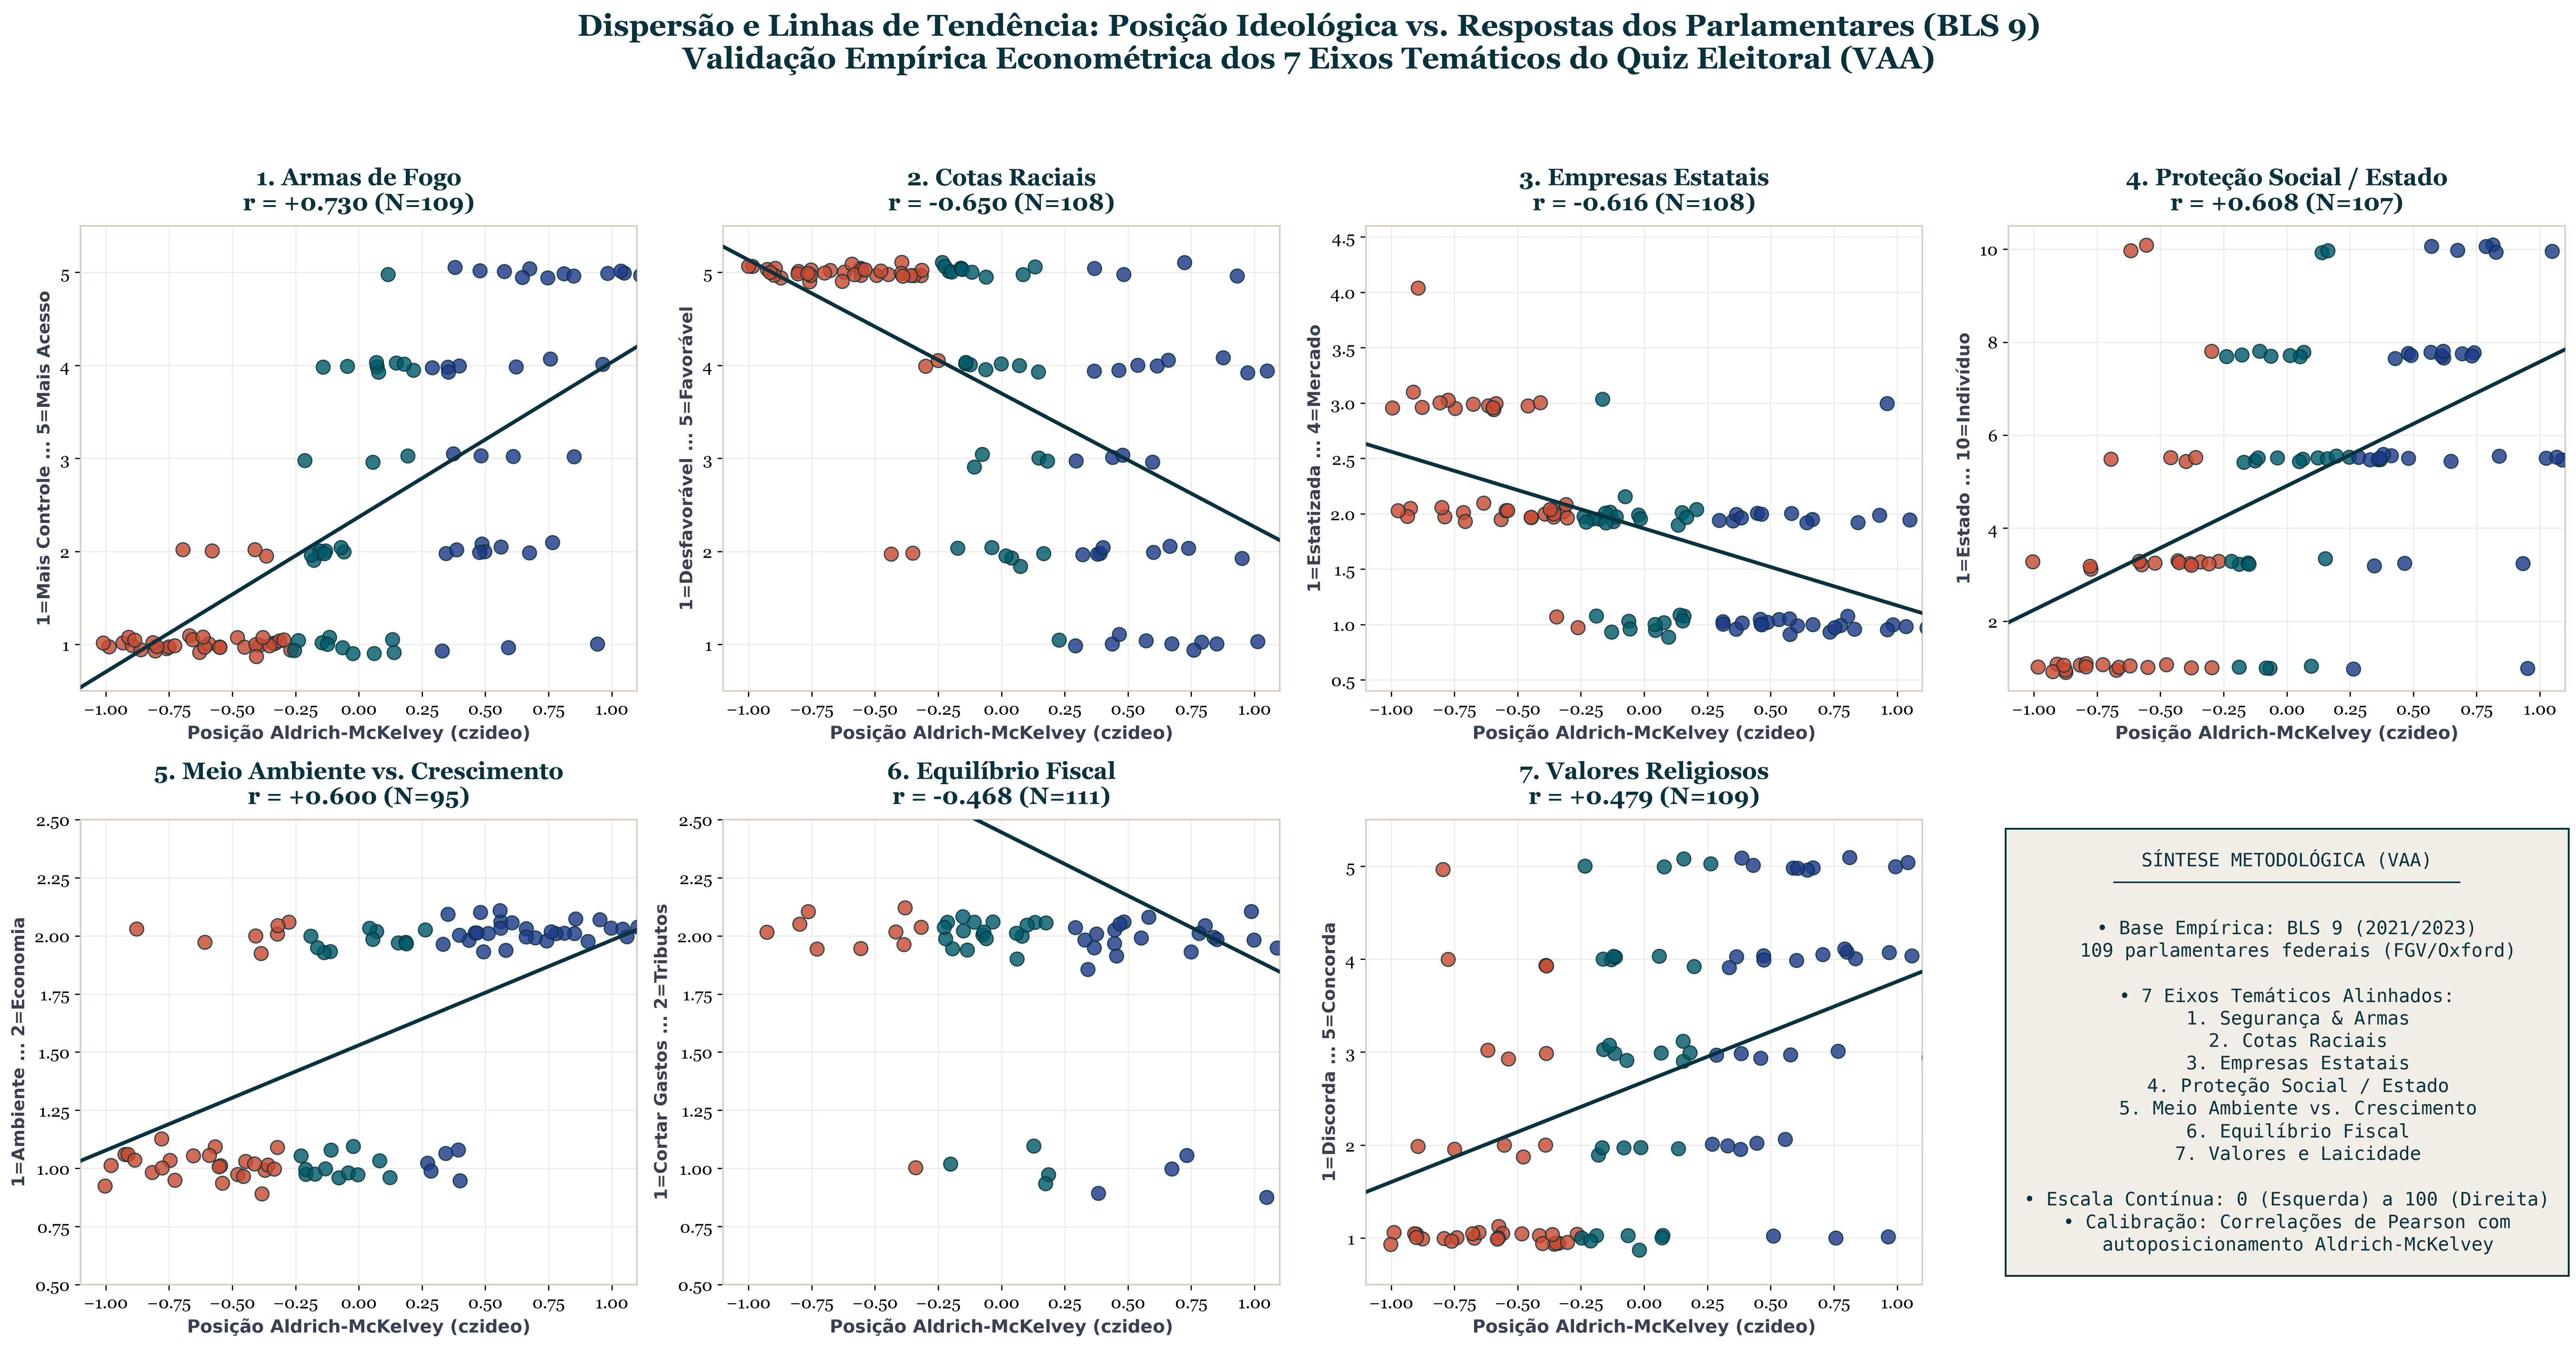
\includegraphics[width=0.90\textwidth]{figures/bls_dispersao_temas.png}
    \caption{\textbf{Painel de Dispersão dos Microdados Legislativos (BLS 9):} Distribuição das respostas individuais dos parlamentares federais ($N=109$) nos 7 eixos temáticos do Quiz e síntese metodológica, acompanhadas de retas de regressão OLS.}
    \label{fig:dispersao}
\end{figure}

\clearpage

% ======================================================================
% PÁGINA 8: TABELA 2 (QUIZ ABNT) E REFERÊNCIAS BIBLIOGRÁFICAS
% ======================================================================
\subsection{Matriz de Perguntas e Pesos do Quiz do Cidadão}

A Tabela~\ref{tab:quiz} detalha as 7 afirmações apresentadas aos usuários, as variáveis correspondentes no banco de dados do BLS e sua correlação matemática com a régua ideológica nacional, apresentada em formato ABNT sem linhas verticais:

\begin{table}[H]
\centering
\caption{\textbf{Matriz de perguntas e coeficientes de correlação do quiz eleitoral}}
\label{tab:quiz}
\vspace{0.4em}
\setlength{\tabcolsep}{4pt}
\small
\renewcommand{\arraystretch}{1.20}
\begin{tabular*}{\textwidth}{@{\extracolsep{\fill}}p{2.6cm} p{7.2cm} c c p{2.4cm}@{}}
\toprule
\textbf{Eixo Temático} & \textbf{Afirmação Apresentada ao Cidadão} & \textbf{Variável} & \textbf{Correlação (r)} & \textbf{Vetor Ideológico} \\
\midrule
\textbf{1. Segurança \& Armas} & O cidadão comum deveria ter maior facilidade para possuir e portar armas de fogo. & \texttt{armas} & +0,730 & \textbf{\color{TagDireita}Direita (+)} \\
\textbf{2. Ações Afirmativas} & Universidades públicas devem manter cotas com critérios étnico-raciais para estudantes negros e indígenas. & \texttt{cotaafro} & -0,650 & \textbf{\color{TagEsquerda}Esquerda (--)} \\
\textbf{3. Papel do Estado} & O Estado deve manter empresas estatais em setores estratégicos da economia, como energia e combustíveis. & \texttt{econlmr} & -0,616 & \textbf{\color{TagEsquerda}Esquerda (--)} \\
\textbf{4. Proteção Social} & O Estado deve ter como papel primordial garantir a proteção social e o bem-estar de todos os cidadãos. & \texttt{govresp} & -0,608 & \textbf{\color{TagEsquerda}Esquerda (--)} \\
\textbf{5. Meio Ambiente} & A preservação ambiental deve ser prioritária, mesmo que limite ou desacelere o crescimento econômico. & \texttt{enviro} & -0,600 & \textbf{\color{TagEsquerda}Esquerda (--)} \\
\textbf{6. Política Fiscal} & O equilíbrio das contas públicas deve ser buscado prioritariamente pelo corte de despesas, e não pelo aumento de impostos. & \texttt{fiscal} & +0,468 & \textbf{\color{TagDireita}Direita (+)} \\
\textbf{7. Valores e Laicidade} & O governo deve promover valores religiosos nas políticas públicas e na educação. & \texttt{valcrist} & +0,479 & \textbf{\color{TagDireita}Direita (+)} \\
\bottomrule
\end{tabular*}
\vspace{0.4em}
\raggedright \footnotesize
\textbf{Fonte:} Elaborado pelos autores a partir dos microdados da 9ª onda do \textit{Brazilian Legislative Survey} (Power \& Zucco Jr., 2023).
\end{table}

\vspace{0.8em}

\section{Referências Bibliográficas}

\begin{itemize}\setlength{\itemsep}{0.3em}
    \item ALDRICH, John H.; McKELVEY, Richard D. A method of scaling with applications to the political issues of the 1970 presidential election. \textbf{American Political Science Review}, v.~71, n.~1, p.~111--130, 1977.
    \item BOLOGNESI, Bruno; RIBEIRO, Ednaldo; CODATO, Adriano. Uma nova classificação ideológica dos partidos políticos brasileiros. \textbf{DADOS --- Revista de Ciências Sociais}, Rio de Janeiro, v.~66, n.~2, e20210164, 2023. DOI: 10.1590/dados.2023.66.2.291.
    \item FOLHA DE S.PAULO / DELTAFOLHA. \textbf{GPS Partidário 2026: Código aberto e dados do GPS ideológico em 5 dimensões}. São Paulo: Repositório GitHub DeltaFolha, 2026.
    \item POWER, Timothy J.; ZUCCO JR., Cesar. Estimating ideology of Brazilian legislative parties, 1990--2005: A research communication. \textbf{Latin American Research Review}, v.~44, n.~1, p.~218--246, 2009.
    \item POWER, Timothy J.; ZUCCO JR., Cesar. \textbf{Brazilian Legislative Survey (Waves 1--9, 1990--2021)}. Harvard Dataverse, Cambridge, 2023. DOI: 10.7910/DVN/WM9IZ.
    \item TRIBUNAL SUPERIOR ELEITORAL (TSE). \textbf{Repositório de Dados Eleitorais: Estatísticas e Candidaturas 2026}. Brasília: TSE, 2026.
\end{itemize}

\vspace{1.5em}
\begin{center}
    {\color{BorderGray}\rule{0.6\textwidth}{1pt}}\\[0.8em]
    \small\color{SlateMuted}\href{https://emquemeuvoto.onrender.com}{emquemeuvoto.onrender.com}
\end{center}

\end{document}
